% Parallel Architectures and GPU Programming chapter (N). Compile from report/.
% Tables: report/tables/*.tex, written by `python -m experiments.report_tables` from committed
% results (rule 11). Bibliography keys (shared .bib): varah1975, meurant2018, shewchuk1994
% (add Shewchuk to CLAUDE.md §16.1 first, §18.6), deepoheatv2, nows2025.

\chapter{Certified solving on the GPU}
\label{ch:pagp}

The gate of Chapter~\ref{ch:dl} needs an exact solver it can call often and a way to stop that
solver as soon as its answer is good enough \emph{with a guarantee}. This chapter describes the
discrete model and its solvers (Section~\ref{sec:pagp-model}), the GPU kernels
(Section~\ref{sec:pagp-kernels}), the error certificate that lets a solve stop early
(Section~\ref{sec:pagp-cert}), the batched certify-on-demand pipeline
(Section~\ref{sec:pagp-batch}) and the 92{,}311-solve labelling job that every gate experiment
rests on (Section~\ref{sec:pagp-oracle}).

\section{Discrete model and solvers}
\label{sec:pagp-model}
The board is discretised with cell-centred finite volumes on a $256\times256$ grid per layer,
four layers, 262{,}144 unknowns. In-plane faces use the harmonic mean of the two cells' sheet
conductances; neighbouring layers are coupled through the dielectric and the vias; convection
acts on the outer faces and heat-sunk edges add a half-cell Dirichlet term. Every cell therefore
has at most seven couplings: the matrix $A$ is a symmetric 7-point layered stencil. Its
off-diagonal entries are non-positive, its rows are weakly diagonally dominant and strictly so
where heat leaves the board, and its coupling graph is connected, so $A$ is a nonsingular
M-matrix (invariant B1, checked on 50 random boards per configuration by
\texttt{solvers/mmatrix\_test.py}). Second-order convergence on manufactured solutions and an
energy balance within 0.1\,\% per board are tested in CI (invariant B2).

Table~\ref{tab:solvers} compares the solvers (E3). A direct sparse factorisation is the
reference; algebraic multigrid (PyAMG, Ruge--St\"uben) preconditioning GMRES is the fastest CPU
solver, about 1.6~s per board when the strength threshold is lowered; preconditioned conjugate
gradients (PCG) needs over 1{,}300 iterations but each one is a stencil application and a few
vector operations, which is what a GPU does well. Stationary Jacobi and red-black Gauss--Seidel
do not converge in their iteration cap. A warm start from the network's prediction lowers the
initial error but barely changes the iteration count to a fixed tolerance, the observation that
motivates certified stopping. The production PCG uses a line-$z$ block-Jacobi preconditioner,
the exact inverse of each column's $4\times4$ tridiagonal block, which is the block-diagonal part
of the symmetric positive definite $A$ and hence SPD, as PCG requires (decision D10).

% generated by experiments/report_tables.py from bench/results/solver_table_v1.csv
\begin{table}[t]\centering\small
\begin{tabular}{llrrr}
\hline
Solver & device & converged & median iterations & median time (s) \\
\hline
jacobi\_gpu & gpu & 0/20 & 1000 & 0.74 \\
rb\_gs\_gpu & gpu & 0/20 & 1000 & 1.06 \\
pyamg\_gmres\_theta0.1 & cpu & 20/20 & 13 & 1.56 \\
pcg\_warm\_gpu & gpu & 20/20 & 1320 & 2.36 \\
pcg\_cold\_gpu & gpu & 20/20 & 1407 & 2.54 \\
jacobi & cpu & 0/20 & 1000 & 3.07 \\
pyamg\_gmres & cpu & 20/20 & 50 & 4.76 \\
pcg\_warm & cpu & 20/20 & 1320 & 6.95 \\
pcg\_cold & cpu & 20/20 & 1407 & 7.33 \\
rb\_gs & cpu & 0/20 & 1000 & 8.85 \\
direct & cpu & 20/20 & 0 & 22.89 \\
\hline
\end{tabular}
\caption{E3: solvers to a true relative residual of $10^{-8}$ on 20 fixed boards at $256^2\times4$ (commit b71e5df). Stationary sweeps are capped and do not converge.}
\label{tab:solvers}
\end{table}


\section{GPU kernels}
\label{sec:pagp-kernels}
The operator is applied matrix-free by Numba CUDA kernels on arrays ordered
$[\text{board},\text{layer},y,x]$, with one thread per cell and thread index $x$ on the
contiguous axis so that loads coalesce. The tiled kernel stages a $16\times16$ tile and its halo
in shared memory; unlike the reference kernel it started from, it also computes the boundary
ring, which the reference skipped. Dot products use a warp-shuffle reduction, and red-black
Gauss--Seidel updates the two colours of the 7-point stencil in turn.

Table~\ref{tab:bw} measures one stencil application. The kernel is memory-bound (a handful of
multiply-adds per nine streamed values), so the figure of merit is achieved bandwidth against the
card's peak. A single board reaches only 5--11\,\% of peak: one launch over 262{,}144 cells is too
small to keep the whole GPU busy. Batching boards fixes this: at 16 and 64 boards in double
precision the kernels reach 77--79\,\% of peak. The tiled kernel gains little over the naive one
at large batches; we did not profile why (a likely reason is that the hardware cache already
serves most neighbour reads). This is the quantitative case for the batched pipeline of
Section~\ref{sec:pagp-batch}.

% generated by experiments/report_tables.py from bench/results/stencil_bw.csv
\begin{table}[t]\centering\small
\begin{tabular}{llrrrr}
\hline
Kernel & dtype & boards $B$ & median ms & GB/s & \% of peak \\
\hline
naive & float32 & 1 & 0.112 & 84 & 5.4 \\
tiled & float32 & 1 & 0.114 & 83 & 5.3 \\
naive & float32 & 16 & 0.324 & 466 & 30.0 \\
tiled & float32 & 16 & 0.227 & 665 & 42.8 \\
naive & float32 & 64 & 0.814 & 742 & 47.7 \\
tiled & float32 & 64 & 0.870 & 694 & 44.7 \\
naive & float64 & 1 & 0.112 & 168 & 10.8 \\
tiled & float64 & 1 & 0.112 & 168 & 10.8 \\
naive & float64 & 16 & 0.257 & 1175 & 75.5 \\
tiled & float64 & 16 & 0.253 & 1192 & 76.7 \\
naive & float64 & 64 & 0.995 & 1214 & 78.1 \\
tiled & float64 & 64 & 0.981 & 1231 & 79.1 \\
\hline
\end{tabular}
\caption{One application of the layered 7-point stencil at $256^2\times4$ on NVIDIA A100-PCIE-40GB (commit 80b752b); peak 1555.2 GB/s from the card's memory clock and bus width (\texttt{docs/refs/a100\_pcie\_40gb\_bandwidth.txt}); bytes model: 9 streams x cells x 4 B.}
\label{tab:bw}
\end{table}


\section{A certificate for early stopping}
\label{sec:pagp-cert}
For a nonsingular M-matrix, $A^{-1}\ge 0$ entrywise. Hence for any $z>0$ with $Az>0$,
\[
  \|A^{-1}\|_\infty \le \hat\kappa := \frac{\max_i z_i}{\min_i (Az)_i},
  \qquad
  \|\theta - x\|_\infty \le \hat\kappa\,\|b - Ax\|_\infty
\]
for any approximation $x$ (Lemma~2(a,b), Appendix~\ref{app:lemmas}); with $z = 1$ this is Varah's
bound \cite{varah1975}, which is useless here because the internal layers have no row margin.
If moreover $w\ge0$ and $Aw\ge|b-Ax|$, then $|\theta-x|\le w$ cell by cell (Lemma~2(c)). The
certificate is computed in double precision with a derived rounding margin
(\texttt{certify/margin.py}, Steps 1--7: every SpMV and residual rounding is bounded, so the
reported number is a guaranteed upper bound on the error to the exact solution of the assembled
system), and it is never formed from the recursive residual of PCG, which drifts.

Two findings changed the construction on the four-layer board. First, $z\approx A^{-1}\mathbf 1$
from three multigrid V-cycles, as planned, gave no certificate at all: on boards without a
heat-sunk edge the V-cycle barely reduces the near-constant mode of $Az=\mathbf 1$, and $Az$ stayed
negative in roughly a third of the cells after 40 cycles. Sixty iterations of conjugate gradients
preconditioned by the same V-cycle give $\min Az$ close to~1 and $\hat\kappa$ within a few per cent
of its exact value (decision ``kappa-hat z by AMG-CG''). Second, the same weakness made the
pointwise certificate loose, and the same fix applies to its first approximation of
$A^{-1}|r|$ (decision ``Pointwise w by AMG-CG''). Validity is unaffected by either change: the
positivity conditions are checked before a certificate is used.

\paragraph{E13: how early can a solve stop?} Table~\ref{tab:e13} runs PCG from the ensemble's
prediction on the 1{,}000 test boards. All 1{,}000 boards obtained a certificate and no bound was
below the true error (invariant B7). Stopping when the error is certified below $\tau_v$ saves
57\,\% of the iterations at 1~K and 43\,\% at 0.1~K with Lemma~2(b) alone
% report/tables/e13.tex (v3-freeze rows)
against solving to the fixed $10^{-8}$; the pre-registered target (H6) was 50\,\% at 0.1~K,
counting the pointwise certificate (decision D1). With the first-generation pointwise certificate
the best saving at 0.1~K is 45\,\%, short of the target, and the week-6 rule asked for the
improved pointwise variant. With its first approximation computed by AMG-CG (second pair of rows,
tag \texttt{v3.4-freeze}), the best certificate saves 79\,\% of the iterations at 1~K and
59\,\% at 0.1~K, % report/tables/e13.tex (v3.4-freeze rows); experiments/results/e13_pwcg
again with every one of the 1{,}000 boards certified and no violation: H6 passes.
The Lemma~2(b) bound is about 200 times the true error at the stop: it bounds every cell by the
worst case of $A^{-1}$, which is large ($\hat\kappa\approx1.5\times10^6$~K/W for a board that
loses heat only by convection). On the $64^2$ single-layer development plate, the same procedure
saves 76--84\,\% at 1~K and 58--62\,\% at 0.1~K with $\hat\kappa$ within 3\,\% of the true norm
(\texttt{bench/results/prelim\_stop.csv}): the four-layer board is markedly harder.

% generated by experiments/report_tables.py from experiments/results/e13/e13_summary.json, experiments/results/e13_pwcg/e13_summary.json
\begin{table}[t]\centering\small
\begin{adjustbox}{max width=\linewidth}\begin{tabular}{llrrrrrr}
\hline
run & $\tau_v$ & iters to $10^{-8}$ & cert.\ 2(b) & cert.\ best & saved 2(b) & saved best & bound/true \\
\hline
v3-freeze & 1~K & 1303 & 554 & 518 & 57\% & 60\% & 178$\times$ \\
v3-freeze & 0.1~K & 1303 & 748 & 722 & 43\% & 45\% & 204$\times$ \\
v3.4-freeze & 1~K & 1303 & 554 & 273 & 57\% & 79\% & 178$\times$ \\
v3.4-freeze & 0.1~K & 1303 & 748 & 541 & 43\% & 59\% & 204$\times$ \\
\hline
\end{tabular}\end{adjustbox}
\caption{E13 on the 1{,}000 test boards, warm-started from the ensemble mean: mean PCG iterations to the fixed relative residual $10^{-8}$ and to a certified error of $\tau_v$ (Lemma 2(b), and the best of 2(b) and the pointwise 2(c)), the saving, and the median ratio of the Lemma 2(b) bound to the true error at the stop. Run v3-freeze computes the pointwise certificate's first approximation $w_0$ by 4 multigrid V-cycles, run v3.4-freeze by AMG-preconditioned CG. Zero violations in every run.}
\label{tab:e13}
\end{table}


\section{Certify on demand: one batched launch}
\label{sec:pagp-batch}
Flagged and audited designs are verified together. \texttt{certify/pcg\_batched.py} runs one
PCG over a batch of boards, each with its own step lengths and a done mask; a finished board's
step is set to zero, so it stops changing while the others continue. Every ten iterations the
true residual of every active board is recomputed in double precision on the device and turned
into a certificate on the host; a flagged board leaves when its certified error is below
$\tau_v$, an audited board when its certified score interval decides the gate's question, and
every board stops at a label-independent cap of 20{,}000 iterations (decision D14).
Single-precision iterations, the plan's first choice, cannot be used here: the residual of a
single-precision iterate is of order $\|A\|\,\|x\|\,2^{-24}$, which with
$\hat\kappa\approx1.5\times10^6$ certifies nothing below about 1~K.

Table~\ref{tab:e4} and Figure~\ref{fig:e4} compare the throughput with the sequential CPU loop
that certifies one board at a time (E4). Every certified board was checked against an oracle
solved to $10^{-10}$, with no violation. The batched GPU pipeline certifies 34.9 times as many
designs per second at a batch of 64, % report/tables/e4.tex
above the tenfold target (H5 passed); even a batch of one is 3.3 times faster, and the gain
saturates beyond 64 boards, consistent with the bandwidth saturation of Table~\ref{tab:bw}.

% generated by experiments/report_tables.py from bench/results/pipeline_bench.csv
\begin{table}[t]\centering\small
\begin{adjustbox}{max width=\linewidth}\begin{tabular}{lrrrr}
\hline
Pipeline & batch & certified designs/s & speed-up & mean PCG iterations \\
\hline
sequential CPU loop & 1 & 0.220 & 1.0 & 776 \\
batched GPU & 1 & 0.734 & 3.3 & 753 \\
batched GPU & 8 & 4.173 & 19.0 & 753 \\
batched GPU & 16 & 6.046 & 27.5 & 753 \\
batched GPU & 32 & 7.038 & 32.1 & 753 \\
batched GPU & 64 & 7.659 & 34.9 & 753 \\
batched GPU & 128 & 7.545 & 34.4 & 753 \\
\hline
\end{tabular}\end{adjustbox}
\caption{E4: certified designs per second at $\tau_v = 0.1$~K (256 test boards, float64 iterations; GPU rate includes host-device transfers). H5: passed.}
\label{tab:e4}
\end{table}


\begin{figure}[t]\centering
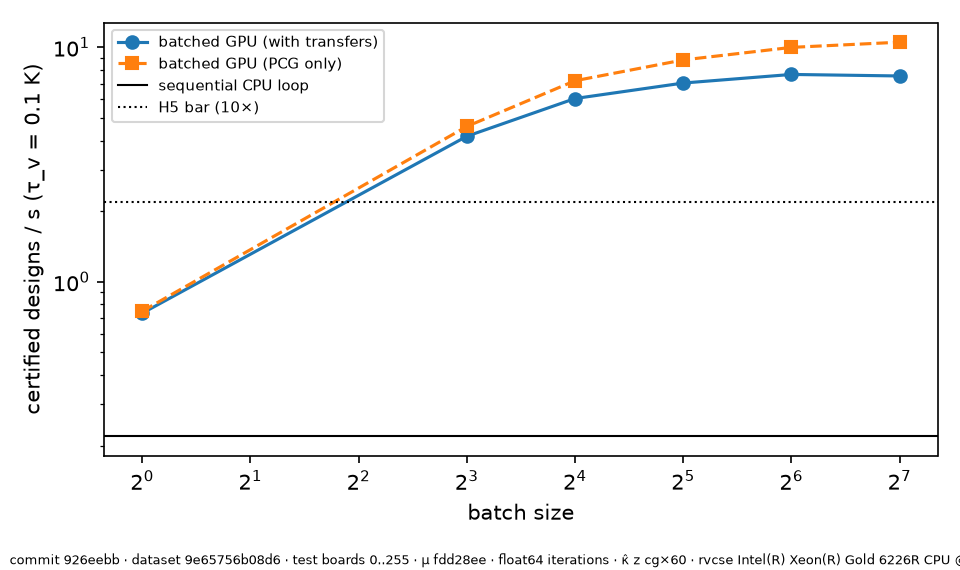
\includegraphics[width=0.8\linewidth]{../bench/figs/pipeline_bench.png}
\caption{E4: certified designs per second against batch size, with the sequential CPU loop and
the H5 bar (footer: commit, data, hardware, date).}
\label{fig:e4}
\end{figure}

\section{The labelling job}
\label{sec:pagp-oracle}
Scoring every gate offline needs the exact peak of all 92{,}311 distinct designs the proposers
produced, solved to $10^{-8}$ (\texttt{experiments/oracle\_label.py}). The first attempt used
60 CPU processes running algebraic multigrid; on a 32-core machine they contended for memory
bandwidth and the throughput was far below the single-process estimate. Moving most of the work
to 16 GPU workers spread over two A100s, each preparing its batch on one core and solving 64
boards per launch in double precision, finished the job at 15.3 boards per second, in 1.6~hours
of wall-clock time and 3.2 GPU-hours held (\texttt{experiments/oracle\_report.md}; the report's
``GPU-hours busy'' row adds overlapping per-worker launch times and overstates GPU use). A
re-solve of a seeded 0.5\,\% of the designs with the other solver agreed to $2.7\times10^{-8}$~K.

\section{Limitations}
\begin{itemize}
\item The certificate holds for the exact solution of the assembled floating-point system;
rounding in the assembly of $A$ is outside the margin.
\item The four-layer board needed AMG-preconditioned CG, not three V-cycles, to construct the
certificate; this adds a few seconds of CPU per design to every verification.
\item The fused gate kernel and a custom scan for stream compaction were planned and not built;
the pipeline uses library compaction.
\item The margin derivation awaits its named checker's sign-off (M), and the certificate
requires the M-matrix property: temperature-dependent conductivity or central-differenced
advection fall outside it.
\end{itemize}
